%%%%%%%%%%%%%%%%%%%%%%%%%%%%%%%%%%%%%%%%%
% Beamer Presentation
% LaTeX Template
% Version 1.0 (10/11/12)
%
% This template has been downloaded from:
% http://www.LaTeXTemplates.com
%
% License:
% CC BY-NC-SA 3.0 (http://creativecommons.org/licenses/by-nc-sa/3.0/)
%
%%%%%%%%%%%%%%%%%%%%%%%%%%%%%%%%%%%%%%%%%

%----------------------------------------------------------------------------------------
%	PACKAGES AND THEMES
%----------------------------------------------------------------------------------------

\documentclass[UTF8,aspectratio=169,14pt]{ctexbeamer}

\usepackage{hyperref}
\hypersetup{
	colorlinks=true,
	linkcolor=red,
	anchorcolor=blue,
	citecolor=green
}

\mode<presentation> {
	
	% The Beamer class comes with a number of default slide themes
	% which change the colors and layouts of slides. Below this is a list
	% of all the themes, uncomment each in turn to see what they look like.
	
	%\usetheme{default}
	%\usetheme{AnnArbor}
	%\usetheme{Antibes}
	%\usetheme{Bergen}
	%\usetheme{Berkeley}
	%\usetheme{Berlin}
	%\usetheme{Boadilla}
	%\usetheme{CambridgeUS}
	%\usetheme{Copenhagen}
	%\usetheme{Darmstadt}
	%\usetheme{Dresden}
	%\usetheme{Frankfurt}
	%\usetheme{Goettingen}
	%\usetheme{Hannover}
	%\usetheme{Ilmenau}
	%\usetheme{JuanLesPins}
	%\usetheme{Luebeck}
	\usetheme{Madrid}
	%\usetheme{Malmoe}
	%\usetheme{Marburg}
	%\usetheme{Montpellier}
	%\usetheme{PaloAlto}
	%\usetheme{Pittsburgh}
	%\usetheme{Rochester}
	%\usetheme{Singapore}
	%\usetheme{Szeged}
	%\usetheme{Warsaw}
	
	% As well as themes, the Beamer class has a number of color themes
	% for any slide theme. Uncomment each of these in turn to see how it
	% changes the colors of your current slide theme.
	
	%\usecolortheme{albatross}
	%\usecolortheme{beaver}
	%\usecolortheme{beetle}
	%\usecolortheme{crane}
	%\usecolortheme{dolphin}
	%\usecolortheme{dove}
	%\usecolortheme{fly}
	%\usecolortheme{lily}
	%\usecolortheme{orchid}
	%\usecolortheme{rose}
	%\usecolortheme{seagull}
	%\usecolortheme{seahorse}
	%\usecolortheme{whale}
	%\usecolortheme{wolverine}
	
	%\setbeamertemplate{footline} % To remove the footer line in all slides uncomment this line
	%\setbeamertemplate{footline}[page number] % To replace the footer line in all slides with a simple slide count uncomment this line
	
	%\setbeamertemplate{navigation symbols}{} % To remove the navigation symbols from the bottom of all slides uncomment this line
}

\usepackage{graphicx} % Allows including images
\graphicspath{{./figs/}}
\usepackage{booktabs} % Allows the use of \toprule, \midrule and \bottomrule in tables
\usepackage{longtable}
\usepackage{listings}
\usepackage{xcolor}
\lstset{numbers=left, %设置行号位置
	numberstyle=\tiny, %设置行号大小
	keywordstyle=\color{blue}, %设置关键字颜色
	commentstyle=\color[cmyk]{1,0,1,0}, %设置注释颜色
	frame=single, %设置边框格式
	escapeinside=``, %逃逸字符(1左面的键),用于显示中文
	%breaklines, %自动折行
	extendedchars=false, %解决代码跨页时,章节标题,页眉等汉字不显示的问题
	xleftmargin=2em,xrightmargin=2em, aboveskip=1em, %设置边距
	tabsize=4, %设置tab空格数
	showspaces=false %不显示空格
}
% Fonts
% \usepackage{libertine}
% \setmonofont{Courier}
\setCJKsansfont[ItalicFont=Noto Serif CJK SC Black, BoldFont=Noto Sans CJK SC Black]{Noto Sans CJK SC}


%----------------------------------------------------------------------------------------
%	TITLE PAGE
%----------------------------------------------------------------------------------------

\title[第1讲]{第1讲 :操作系统概述} % The short title appears at the bottom of every slide, the full title is only on the title page
\subtitle{第五节:OS实验概述}
\author{向勇、陈渝、李国良} % Your name
\institute[清华大学] % Your institution as it will appear on the bottom of every slide, may be shorthand to save space
{
清华大学计算机系 \\ % Your institution for the title page
\medskip
\textit{xyong,yuchen@tsinghua.edu.cn} % Your email address
}
\date{\today} % Date, can be changed to a custom date

\begin{document}

\begin{frame}
\titlepage % Print the title page as the first slide
\end{frame}

%\begin{frame}
%\frametitle{提纲} % Table of contents slide, comment this block out to remove it
%\tableofcontents % Throughout your presentation, if you choose to use \section{} and \subsection{} commands, these will automatically be printed on this slide as an overview of your presentation
%\end{frame}
%
%%----------------------------------------------------------------------------------------
%%	PRESENTATION SLIDES
%%----------------------------------------------------------------------------------------
%
%%------------------------------------------------
%\section{第八节:OS实验概述} % Sections can be created in order to organize your presentation into discrete blocks, all sections and subsections are automatically printed in the table of contents as an overview of the talk
%%------------------------------------------------


\begin{frame}

\frametitle{OS实验概述}

\begin{itemize}
\item 设计思路
    \begin{itemize}
    \item 设计ucore/rcore,覆盖操作系统的关键点,内容如下:
    \begin{itemize}
        \item 外设:I/O管理/中断管理
        \item 内存:虚存管理/页表/缺页处理/页替换算法
        \item CPU:进程管理/调度器算法
        \item 并发:信号量实现和同步互斥应用
        \item 存储:文件系统+磁盘驱动
    \end{itemize}
    \item 完整代码量控制在4000行左右 (希望)
    \item 提供实验讲义和源码分析文档
    \end{itemize}
\end{itemize}

\end{frame}


\begin{frame}[plain]
	
	\frametitle{OS实验内容}

	\begin{columns}[t]
    \begin{column}{.5\textwidth}
     \\
     OS实验内容
     
	\begin{enumerate}
	    \item hello-world OS
		\item kernel-mode OS
		\item multi-programming OS	
		\item mem-isolation OS
		\item multi-process OS
		\item Inter-Process-Comm OS
		\item File-System OS
		\item r/u Core OS
	\end{enumerate}
	\end{column}
	
	\begin{column}{.5\textwidth}
	\begin{figure}
		\centering
		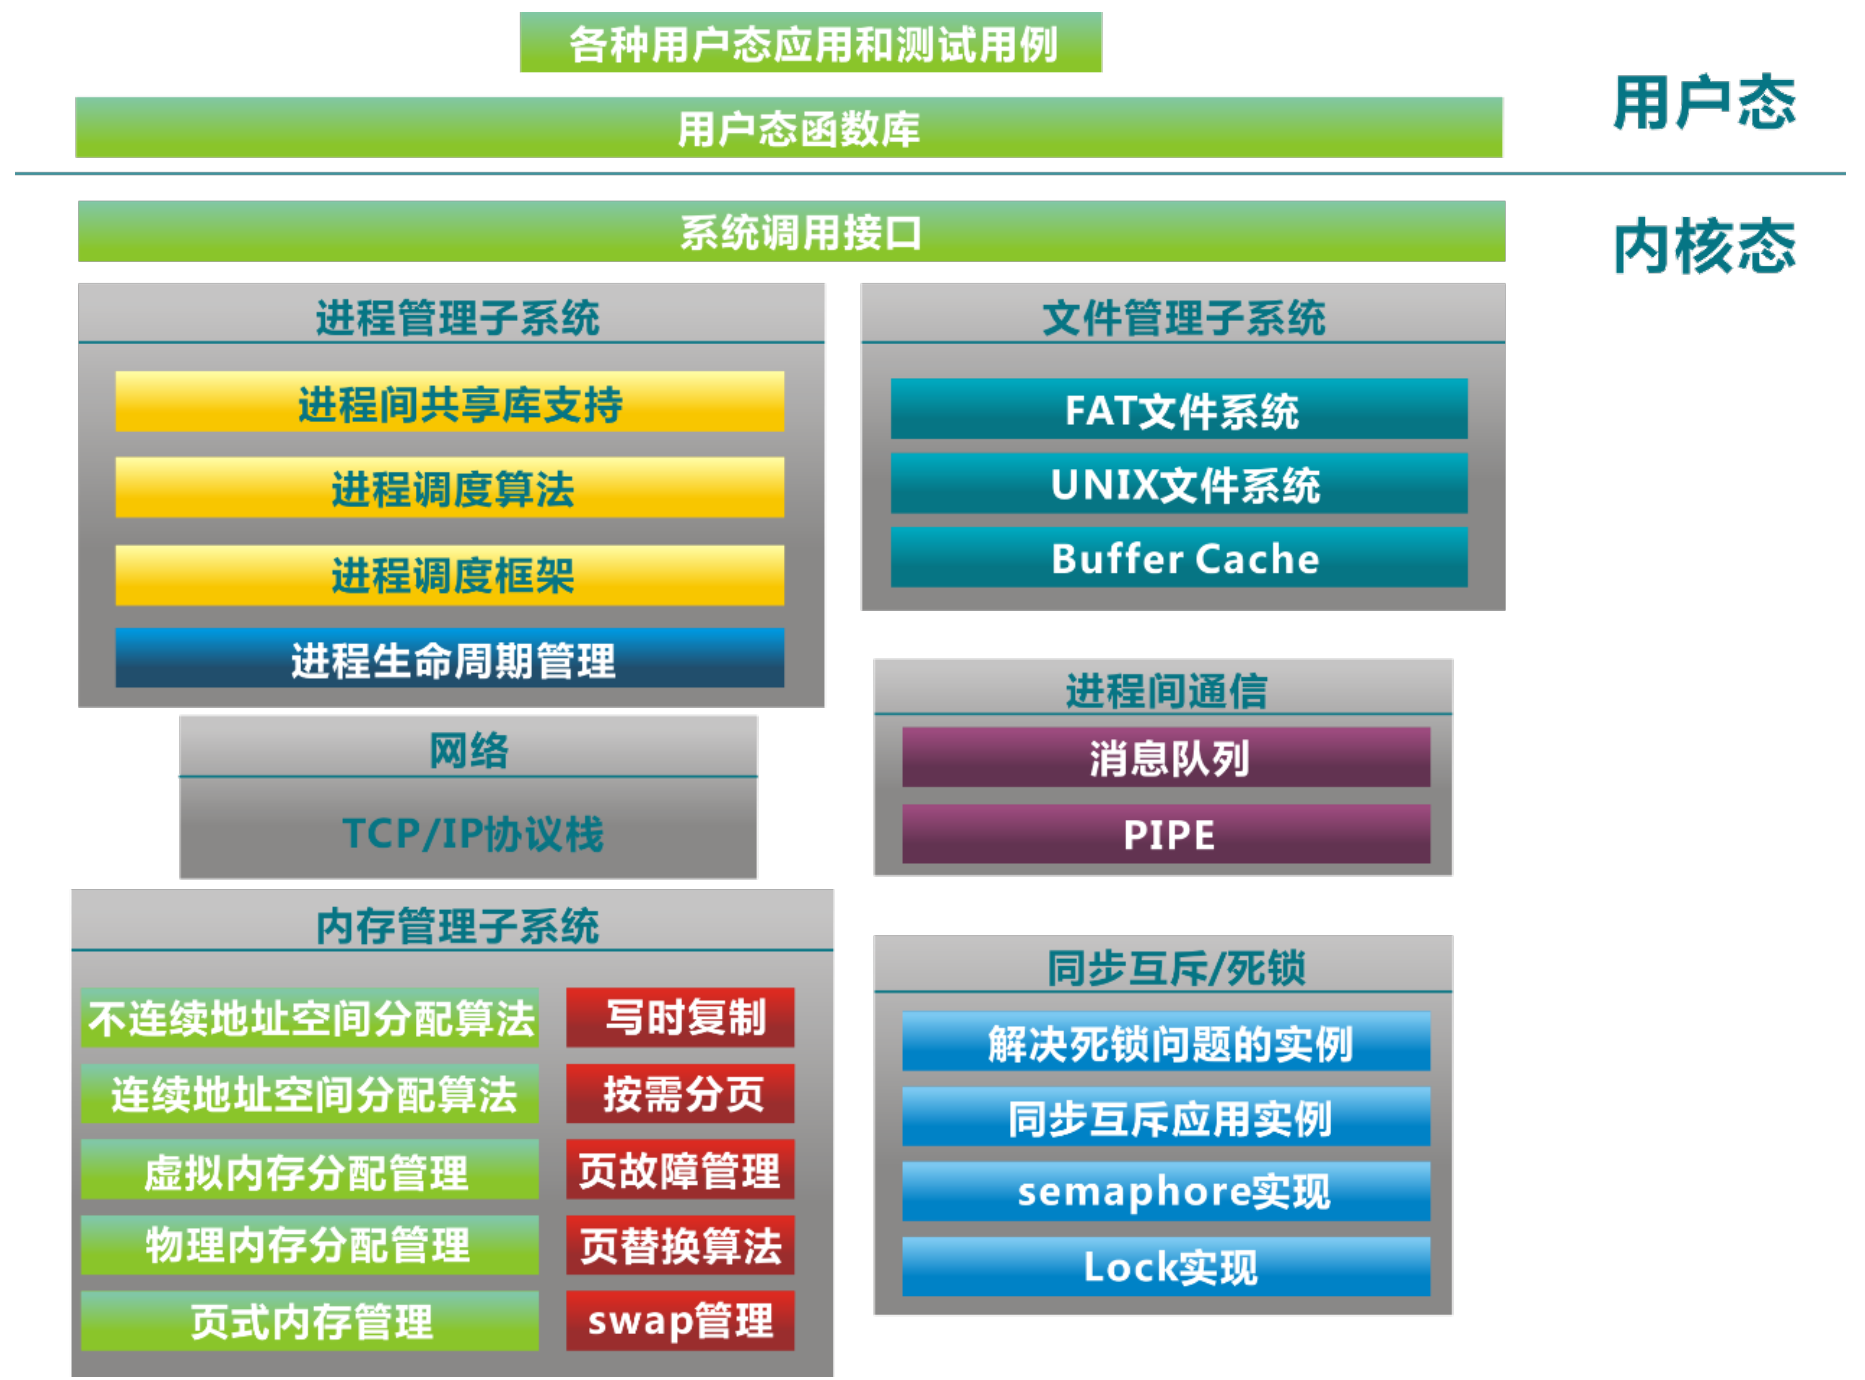
\includegraphics[width=1.0\linewidth]{oslab-overview}
		\caption{OS实验框架}
	\end{figure}
	\end{column}
	\end{columns}
\end{frame}


\begin{frame}
\frametitle{OS实验内容}
\framesubtitle{lab1}
\begin{block}{Lab1:  hello-world OS}
在裸机上的执行环境,让应用与硬件隔离,简化了应用访问硬件的难度和复杂性。
\end{block}

\begin{itemize}
    \item 直接与硬件交互的系统程序的编译运行
    \item 输出字符的方法
    \item 调试系统程序的方法
\end{itemize}
    
\end{frame}


\begin{frame}
\frametitle{OS实验内容}
\framesubtitle{lab2}

\begin{block}{Lab2:  kernel-mode OS}
操作系统利用硬件特权级机制,实现对操作系统自身的保护。
应用在用户态通过系统调用得到内核态的内核服务。
操作系统批处理机制支持多个程序的自动加载和运行。
\end{block}

\begin{itemize}
    \item 特权级机制
    \item 应用程序实现
    \item 批处理机制
    \item 特权级切换
\end{itemize}

\end{frame}

\begin{frame}
\frametitle{OS实验内容}
\framesubtitle{lab3}

\begin{block}{Lab3:multi-programming OS}
操作系统通过协作机制/抢占机制支持程序主动/被动放弃处理器,提高系统效率。
\end{block}

\begin{itemize}
    \item 多道程序的放置与加载
    \item 任务切换
    \item 协作式调度
    \item 抢占式调度    
\end{itemize}

\end{frame}

\begin{frame}
\frametitle{OS实验内容}
\framesubtitle{lab4}

\begin{block}{Lab4: mem-isolation OS}
操作系统通过动态内存分配机制、页表的虚实内存映射机制,
加强内存安全,简化应用开发。
\end{block}

\begin{itemize}
    \item 动态内存分配
    \item 地址空间(Address Space)抽象
    \item 多级页表
\end{itemize}

\end{frame}


\begin{frame}
\frametitle{OS实验内容}
\framesubtitle{lab5}

\begin{block}{Lab5: multi-process OS}
操作系统建立了进程创建、执行、切换和结束的动态管理过程

\end{block}

\begin{itemize}
    \item 进程(Process)抽象
    \item 进程管理
\end{itemize}

\end{frame}

\begin{frame}
\frametitle{OS实验内容}
\framesubtitle{lab6}

\begin{block}{Lab6:Inter-Process-Comm OS}
操作系统通过进程间通信(Inter-Process-Comm)机制,让应用之间建立了有效的联系。
\end{block}

\begin{itemize}
    \item 进程间通信机制
    \item 管道(PIPE)机制
\end{itemize}

\end{frame}


\begin{frame}
\frametitle{OS实验内容}
\framesubtitle{lab7}

\begin{block}{Lab7:File-System OS}
操作系统通过文件系统完成对程序和数据的持久保存与灵活的访问
\end{block}

\begin{itemize}
    \item 文件(File)抽象
    \item 基于inode方式的文件系统的设计与实现
\end{itemize}

\end{frame}


\begin{frame}
\frametitle{OS实验内容}
\framesubtitle{lab8}

\begin{block}{Lab8:r/u Core OS}
为支持更丰富的应用需求,操作系统需要改进与完善。
通过完成一个完整的OS kernel的设计与实现,形成面向操作系统的系统思维。
\end{block}

\begin{itemize}
    \item 操作系统各组成部分关联关系的完善
    \item 操作系统各组成部分的改进与优化
    \item 对应用的进一步服务与支持
\end{itemize}

\end{frame}


\begin{frame}[plain]
\frametitle{OS实验内容}
\framesubtitle{labX}

\begin{block}{LabX:大实验}
前提:已经完成基本实验 \\
尝试完成一些有一定挑战性且有趣的OS实验。
\end{block}

\begin{itemize}
    \item 参加OS比赛的推荐项目
    \item 改进与设计rcore/zcore/acore操作系统
    \item 在一个OS(如Linux)实现一个Hypervisor
    \item 基于异步机制的新型OS
    \item 支持动态更新的OS
    \item 驱动程序运行在用户态的OS
\end{itemize}

\end{frame}


\begin{frame}
	\frametitle{OS实验内容}
	\framesubtitle{labX}
	
\begin{longtable}[]{@{}|l|l|@{}}
	\toprule
	选题方向 & 大实验题目\tabularnewline
	\midrule
	\endhead
	RISC-V &
	\href{https://www.bilibili.com/video/BV1Yy4y1e7zR?p=24}{rCore:Rust操作系统内核的探索+MadFS}\tabularnewline  \hline
	RISC-V &
	\href{http://os.cs.tsinghua.edu.cn/oscourse/OS2019spring/projects/g01}{ucore
		on RISC-V}\tabularnewline  \hline
	RISC-V &
	\href{http://os.cs.tsinghua.edu.cn/oscourse/OS2019spring/projects/g02}{简易版
		rcore 开发与教学文档编写 \&\& rcore plus 开发}\tabularnewline \hline
	RISC-V &
	\href{http://os.cs.tsinghua.edu.cn/oscourse/OS2019spring/projects/g05}{FPGA
		上运行 RISC-V rCore 构建路由器}\tabularnewline \hline
	x86\_64 &
	\href{http://os.cs.tsinghua.edu.cn/oscourse/OS2019spring/projects/g04}{对标
		Biscuit OS 真实应用真实网卡及性能测试}\tabularnewline \hline
	x86\_64 &
	\href{http://os.cs.tsinghua.edu.cn/oscourse/OS2019spring/projects/g06}{rCore
		内核可加载模块和动态链接库}\tabularnewline \hline
	MIPS &
	\href{http://os.cs.tsinghua.edu.cn/oscourse/OS2019spring/projects/g03}{第三届全国大学生系统能力培养大赛}\tabularnewline \hline
	Arm &
	\href{http://os.cs.tsinghua.edu.cn/oscourse/OS2019spring/projects/g11}{Python
		(and more) on rCore on RPi}\tabularnewline \hline
	GUI &
	\href{http://os.cs.tsinghua.edu.cn/oscourse/OsTrain2019/g2}{GUI}\tabularnewline \hline
	GUI & \href{http://os.cs.tsinghua.edu.cn/oscourse/OsTrain2019/g3}{适配
		mini GUI}\tabularnewline \hline

	
	\bottomrule
\end{longtable}


\end{frame}



\begin{frame}
	\frametitle{OS实验内容}
	\framesubtitle{labX}
	
	\begin{longtable}[]{@{}|l|l|@{}}
		\toprule
		选题方向 & 大实验题目\tabularnewline
		\midrule
		\endhead
		内核语言 &
		\href{http://os.cs.tsinghua.edu.cn/oscourse/OsTrain2019/g6}{编译原理/操作系统综合实验}\tabularnewline \hline
		驱动 &
		\href{http://os.cs.tsinghua.edu.cn/oscourse/OsTrain2019/g4}{IO复用}\tabularnewline \hline
		rust &
		\href{http://os.cs.tsinghua.edu.cn/oscourse/OS2019spring/projects/g08}{Audio
			support for rCore}\tabularnewline \hline
		错误分析 &
		\href{http://os.cs.tsinghua.edu.cn/oscourse/OS2019spring/projects/g07}{在ucore获得稳定触发竞争条件的漏洞样本}\tabularnewline \hline
		行为分析 &
		\href{http://os.cs.tsinghua.edu.cn/oscourse/OS2019spring/projects/g09}{Program
			Analysis via Memory Access Patterns}\tabularnewline \hline
		微内核 &
		\href{http://os.cs.tsinghua.edu.cn/oscourse/OsTrain2019/g1}{调研Fuchsia的微内核,尝试rcore微内核的修改}\tabularnewline \hline
		内核可加载模块 &
		\href{http://os.cs.tsinghua.edu.cn/oscourse/OsTrain2019/g5}{rethink用户/内核态}\tabularnewline \hline
		模拟器 &
		\href{http://os.cs.tsinghua.edu.cn/oscourse/OS2019spring/projects/g10}{操作系统中常用算法的性能分析及优化}\tabularnewline \hline
		教学实验设计 &
		\href{http://os.cs.tsinghua.edu.cn/oscourse/OsTrain2019/g7}{对简易版rcore的进一步维护和更新}\tabularnewline \hline
		\bottomrule
	\end{longtable}
	

\end{frame}
%----------------------------------------------------------------------------------------
\begin{frame}
    \frametitle{OS实验内容}
    \framesubtitle{lab1: hello-world OS}
    \begin{block}{Lab1:  hello-world OS}
        在裸机上的执行环境,让应用与硬件隔离,简化了应用访问硬件的难度和复杂性。
    \end{block}
    
    %    \begin{itemize}
    %        \item 直接与硬件交互的系统程序的编译运行
    %        \item 输出字符的方法
    %        \item 调试系统程序的方法
    %    \end{itemize}
    \begin{figure}
        \centering
        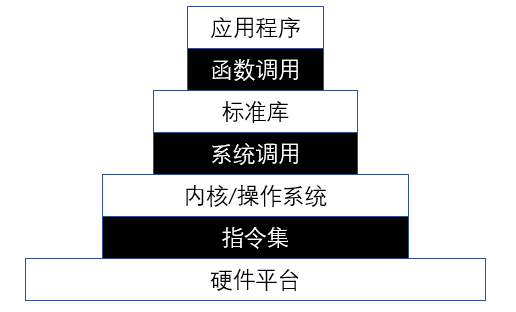
\includegraphics[width=0.6\linewidth]{app-software-stack} %\pause
        %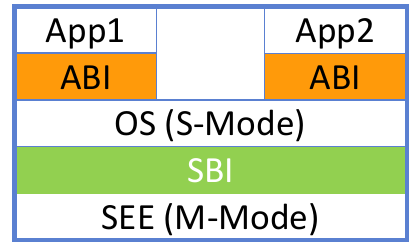
\includegraphics[width=0.4\linewidth]{sbi}
    \end{figure}
    
\end{frame}
%----------------------------------------------------------------------------------------
\begin{frame}
    \frametitle{OS实验内容}
    \framesubtitle{lab1: hello-world OS}
    \begin{block}{Lab1:  hello-world OS}
        在裸机上的执行环境,让应用与硬件隔离,简化了应用访问硬件的难度和复杂性。
    \end{block}
    
    %    \begin{itemize}
    %        \item 直接与硬件交互的系统程序的编译运行
    %        \item 输出字符的方法
    %        \item 调试系统程序的方法
    %    \end{itemize}
    \begin{figure}
        \centering
        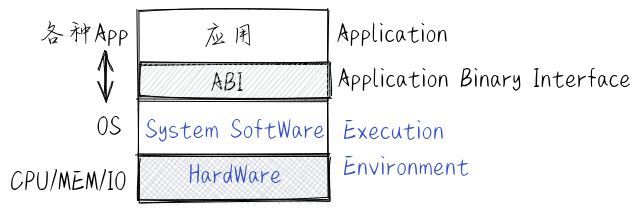
\includegraphics[width=0.55\linewidth]{EE} %\pause
        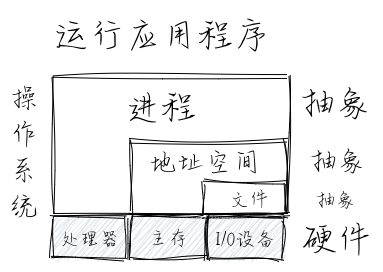
\includegraphics[width=0.4\linewidth]{run-app}
    \end{figure}
    
\end{frame}

%----------------------------------------------------------------------------------------
\begin{frame}
    \frametitle{OS实验内容}
    \framesubtitle{lab1: hello-world OS}
    \begin{block}{Lab1:  hello-world OS}
        在裸机上的执行环境,让应用与硬件隔离,简化了应用访问硬件的难度和复杂性。
    \end{block}
    
    %    \begin{itemize}
    %        \item 直接与硬件交互的系统程序的编译运行
    %        \item 输出字符的方法
    %        \item 调试系统程序的方法
    %    \end{itemize}
    \begin{figure}
        \centering
        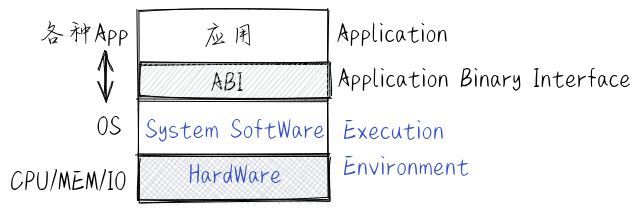
\includegraphics[width=0.55\linewidth]{EE} %\pause
        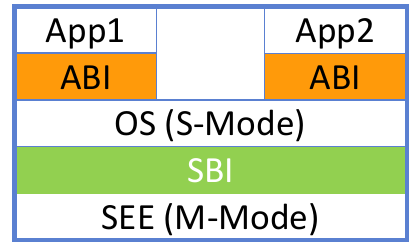
\includegraphics[width=0.4\linewidth]{sbi}
    \end{figure}
    
\end{frame}
%----------------------------------------------------------------------------------------
\begin{frame}
    \frametitle{OS实验内容}
    \framesubtitle{lab1: hello-world OS 硬件}
    

    应用所在的硬件环境:QEMU RISC-V 64虚拟计算机 或 K210 RISC-V 64物理计算机
    \begin{itemize}
        \item 输入输出和存储外设:16550A UART和virtio-block设备
        \item 内存:可参数化的RAM内存(8MB)
        \item CPU:可配置的多核 RV64GC M/S/U mode CPU(1 or 2)
    \end{itemize}
\end{frame}
%----------------------------------------------------------------------------------------
\begin{frame}
    \frametitle{OS实验内容}
    \framesubtitle{lab1: hello-world OS 物理内存}
    
    
    %应用所在的硬件环境:QEMU RISC-V 64虚拟计算机 或 K210 RISC-V 64物理计算机
    \begin{figure}
    \centering
    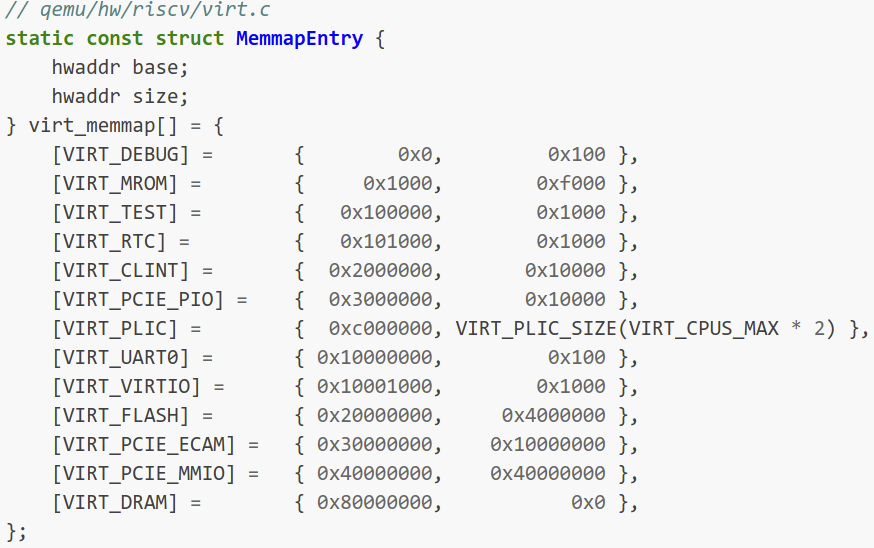
\includegraphics[width=0.75\linewidth]{qemu-mem} %\pause
    %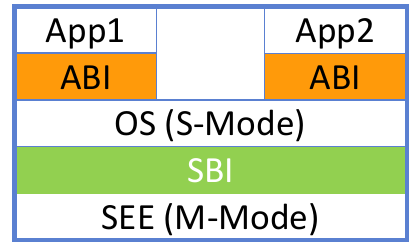
\includegraphics[width=0.4\linewidth]{sbi}
\end{figure}
\end{frame}
%----------------------------------------------------------------------------------------
\begin{frame}
    \frametitle{OS实验内容: 硬件: RISC-V CPU启动}
    %	\framesubtitle{QEMU}
    \centering
    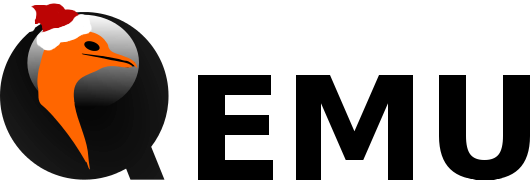
\includegraphics[width=0.2\linewidth]{qemu}	
    \begin{itemize}
        
        \item RISC-V CPU 启动过程
        \begin{itemize}
            \item 初始化CPU/Regs	
            \item 初始化内存
            \item 初始化基本外设
            \item 执行ROM中固化的代码
        \end{itemize}
        \item 出处: \href{https://github.com/qemu/qemu}{https://github.com/qemu/qemu}
        
    \end{itemize}	
    
\end{frame}

%----------------------------------------------------------------------------------------
\begin{frame}[plain]
    %	\frametitle{RISC-V CPU 启动过程--初始化CPU}
    %	\framesubtitle{QEMU}
    %	\centering
    %	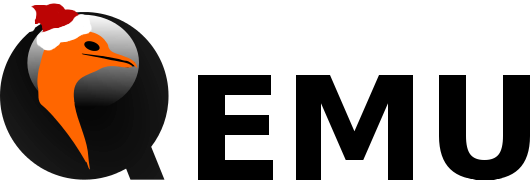
\includegraphics[width=0.1\linewidth]{qemu}	
    %	\begin{itemize}
    %		
    %		\item RISC-V CPU 启动过程--初始化CPU
    %		
    %	\end{itemize}		
    \centering
    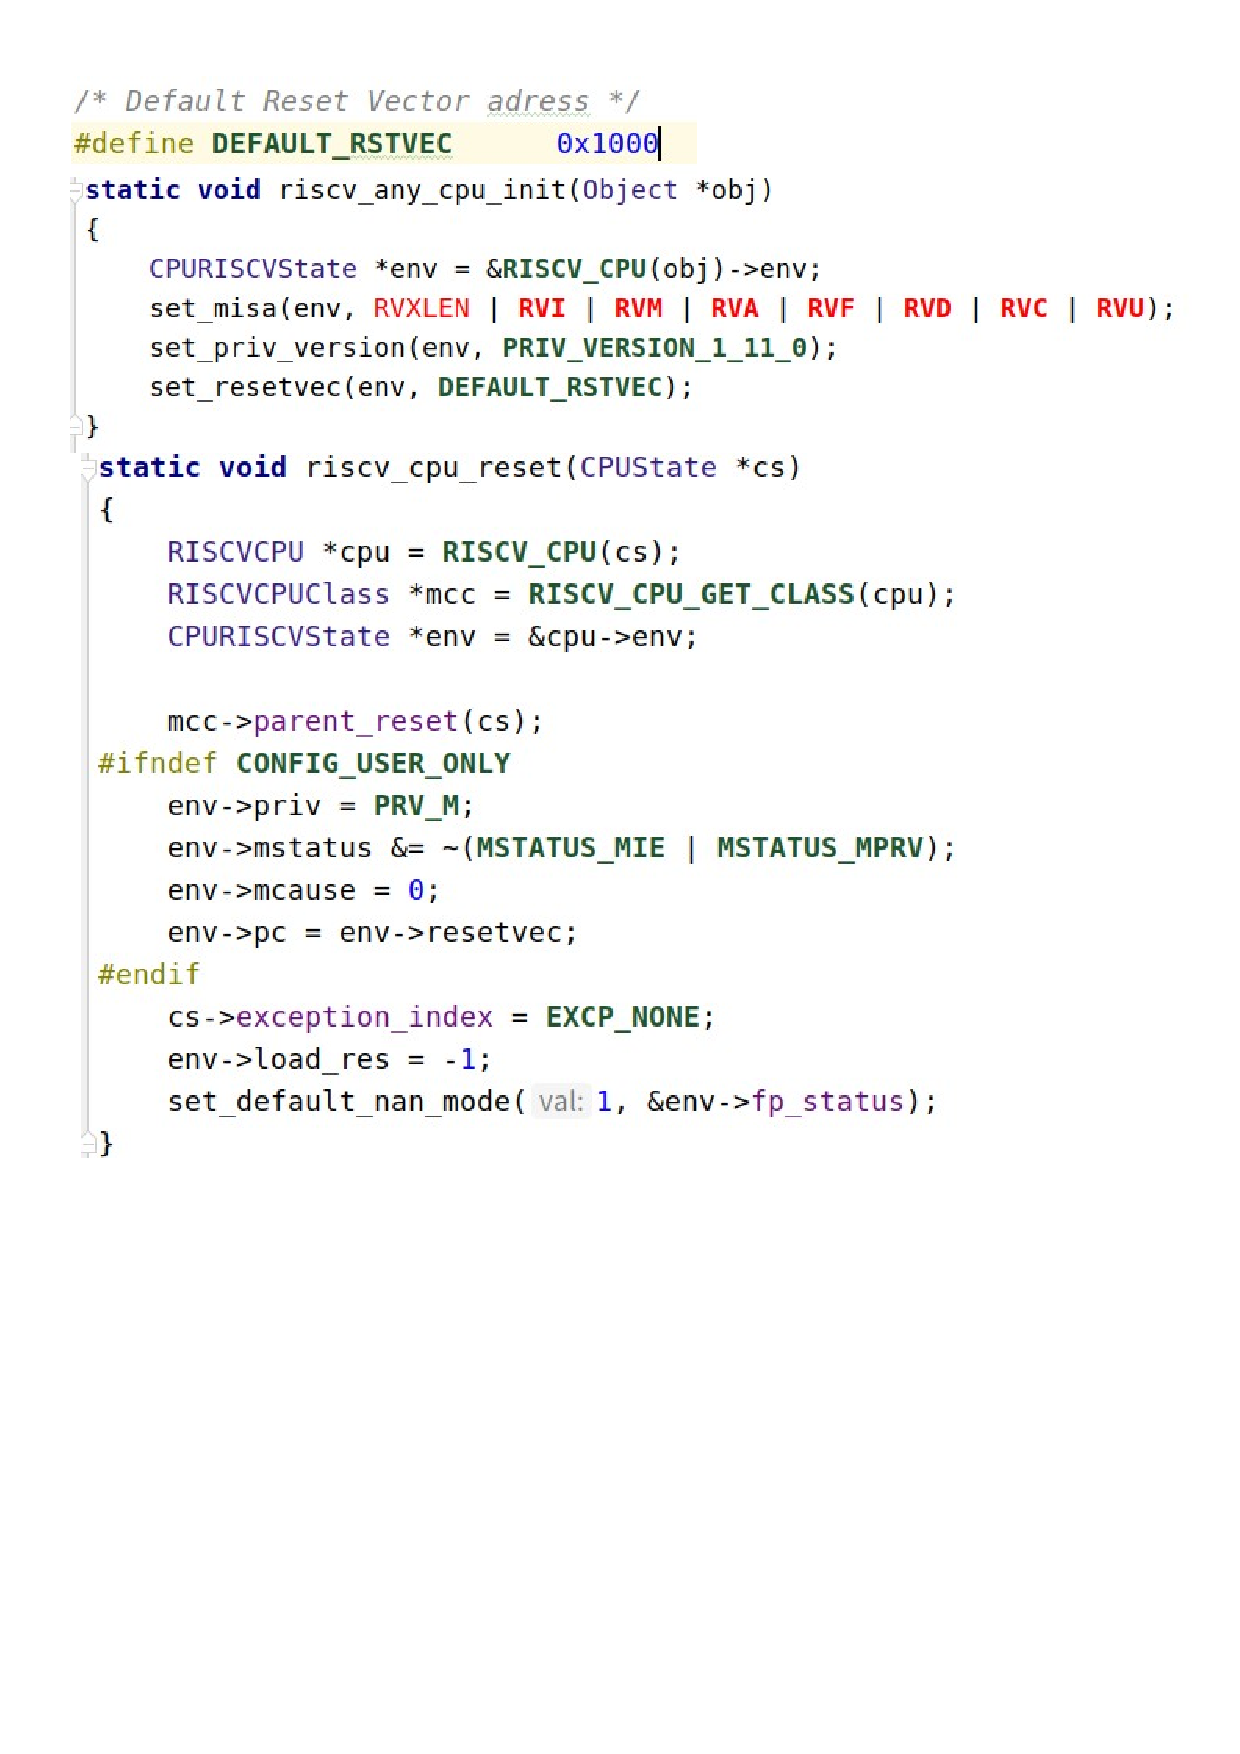
\includegraphics[width=0.65\linewidth]{qemu-initcpu}
\end{frame}

\begin{frame}
    \frametitle{OS实验内容: 硬件: RISC-V CPU启动}
    %	\framesubtitle{QEMU}
    %	\centering
    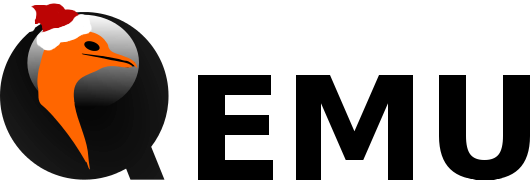
\includegraphics[width=0.1\linewidth]{qemu}	
    \begin{itemize}
        
        \item RISC-V CPU 启动过程--初始化内存
        
    \end{itemize}	
    
    \centering
    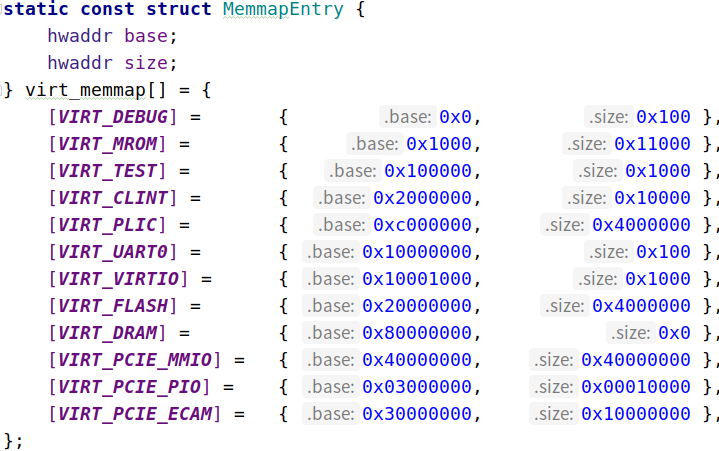
\includegraphics[width=0.6\linewidth]{qemu-initmem}
\end{frame}

\begin{frame}[plain]
    %	\frametitle{ RISC-V CPU 启动过程--初始化外设}
    %	\framesubtitle{QEMU}
    %	\centering
    %	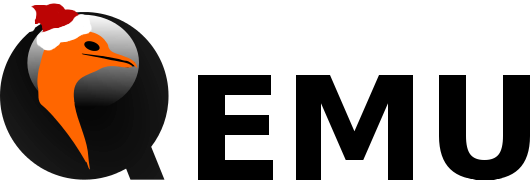
\includegraphics[width=0.1\linewidth]{qemu}	
    %	\begin{itemize}
    %		
    %		\item RISC-V CPU 启动过程--初始化外设
    %		
    %	\end{itemize}	
    \centering
    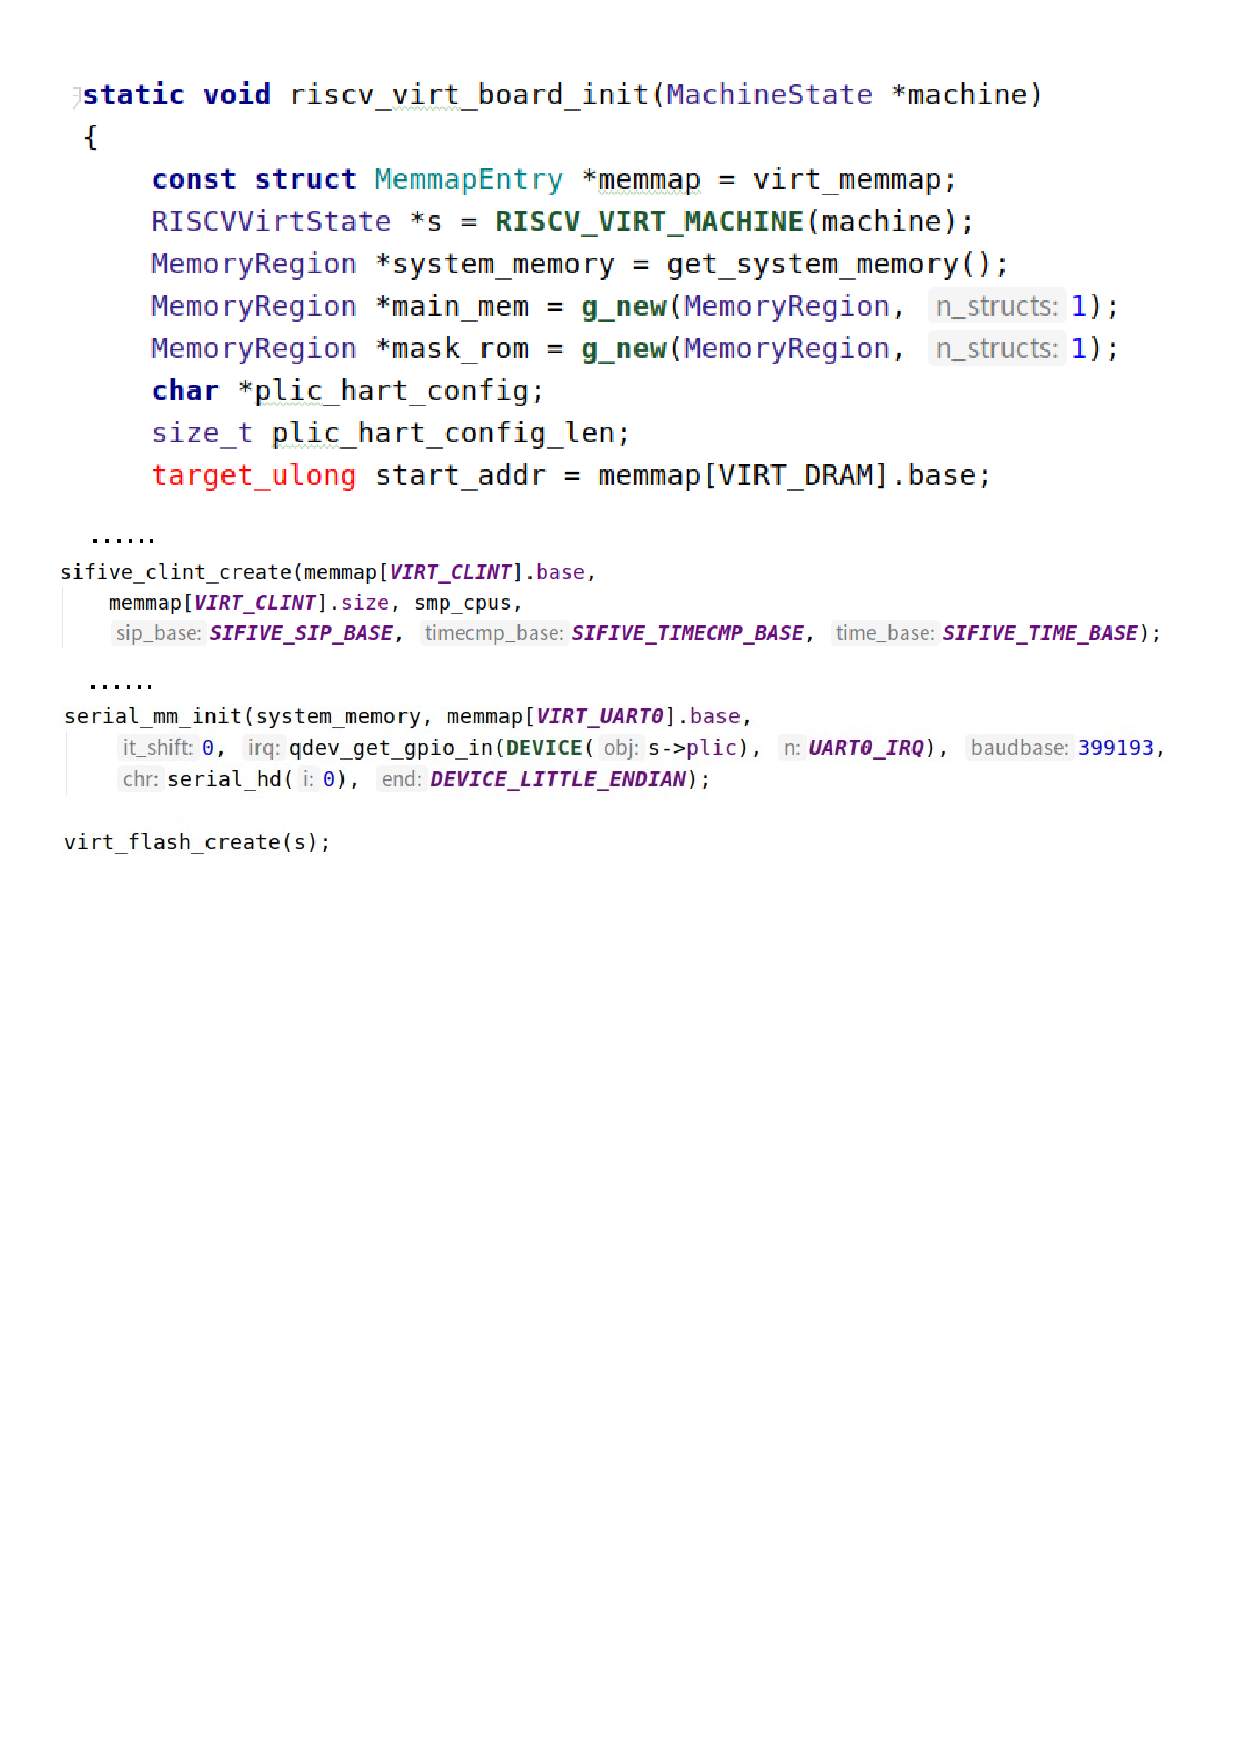
\includegraphics[width=0.8\textwidth]{qemu-initboard}
\end{frame}


\begin{frame}[plain]
    \frametitle{OS实验内容: 硬件: RISC-V CPU启动--ROM初始化代码}
    %	\framesubtitle{QEMU}
    %	\centering
    %	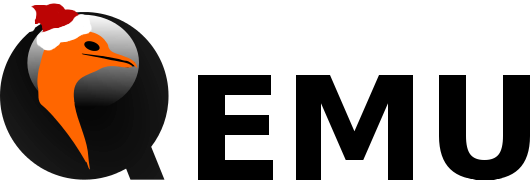
\includegraphics[width=0.1\linewidth]{qemu}	
    %	\begin{itemize}
    %		
    %		\item RISC-V CPU 启动过程--ROM初始化代码
    %		
    %	\end{itemize}	
    
    \centering
    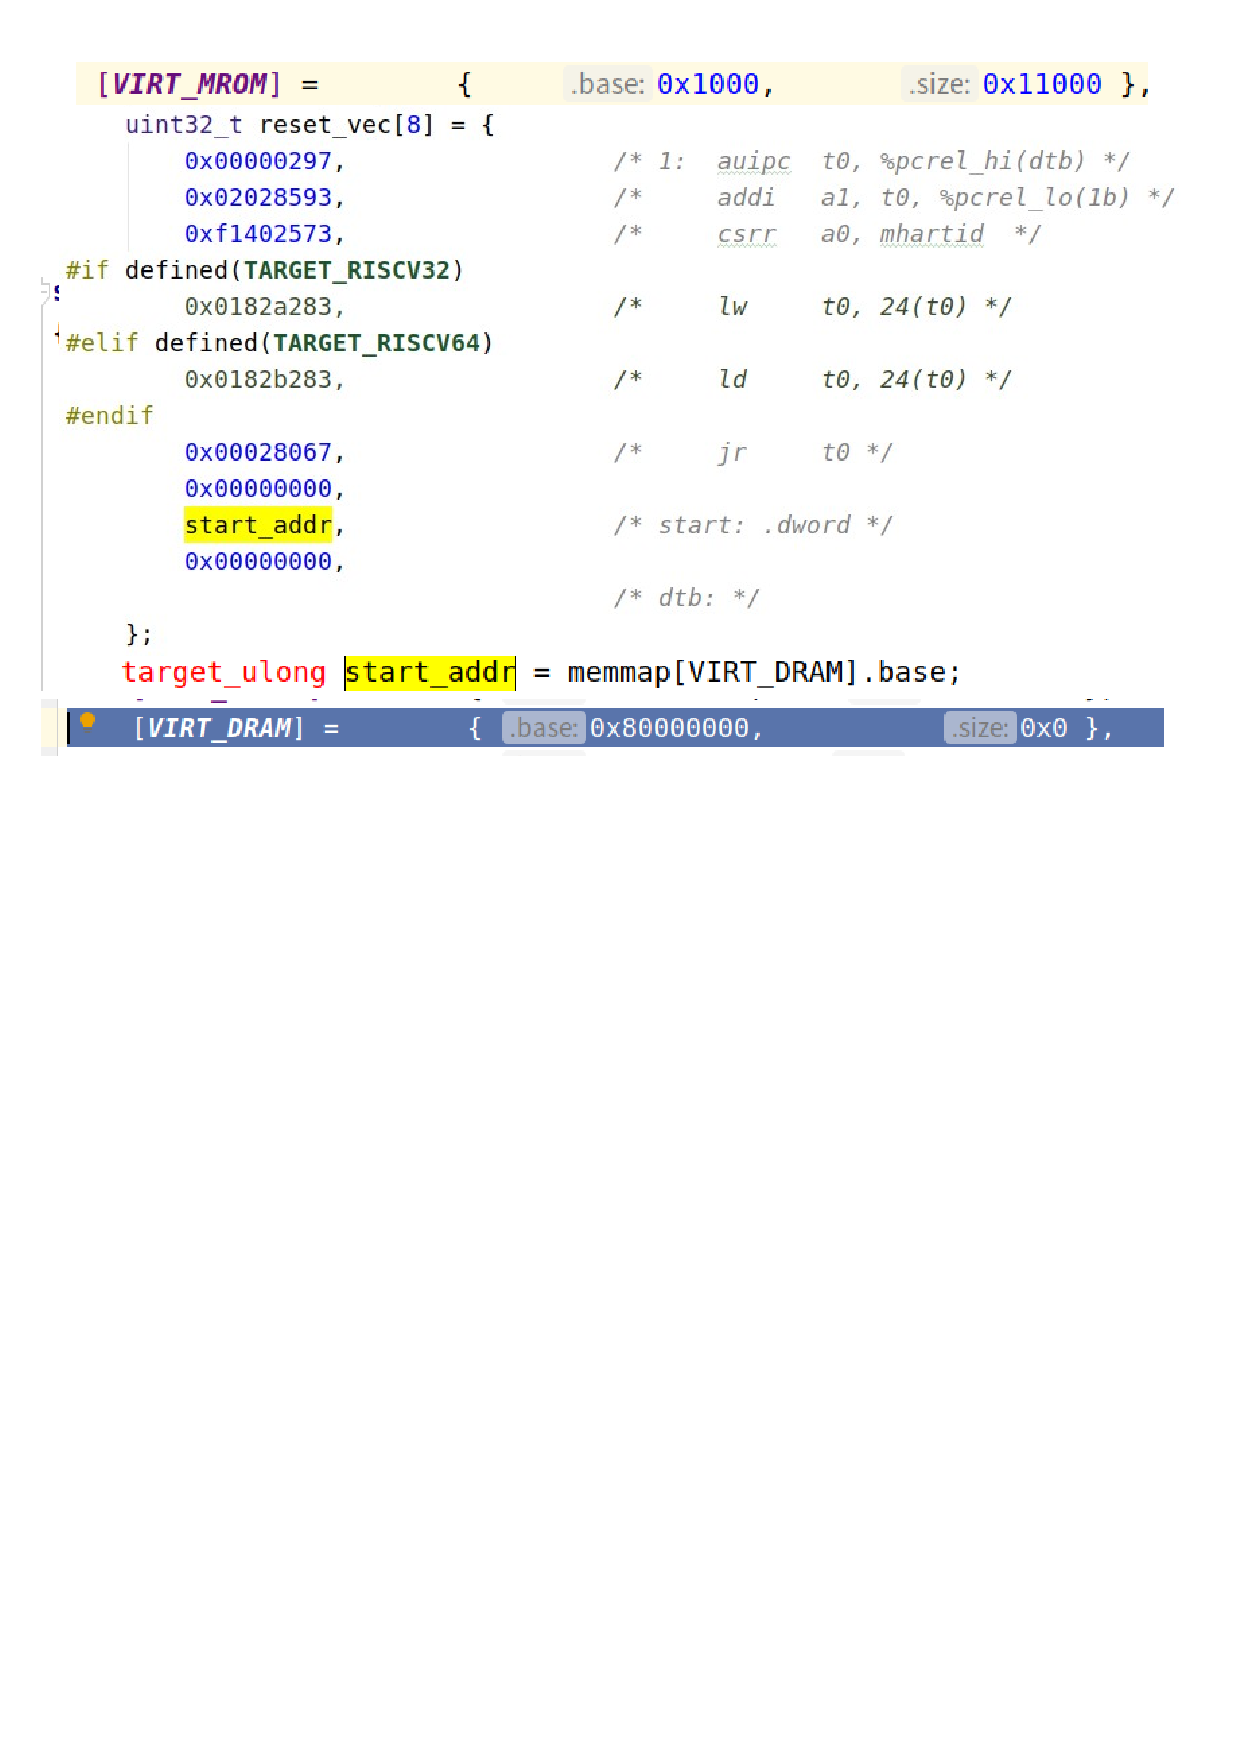
\includegraphics[width=0.8\linewidth]{qemu-resetcode}
\end{frame}


%----------------------------------------------------------------------------------------
\begin{frame}
    \frametitle{OS实验内容}
    \framesubtitle{lab1: hello-world OS  软件}
    
    %    \begin{itemize}
    %        \item 直接与硬件交互的系统程序的编译运行
    %        \item 输出字符的方法
    %        \item 调试系统程序的方法
    %    \end{itemize}
    编译后的应用与运行时的应用
    \begin{figure}
        \centering
        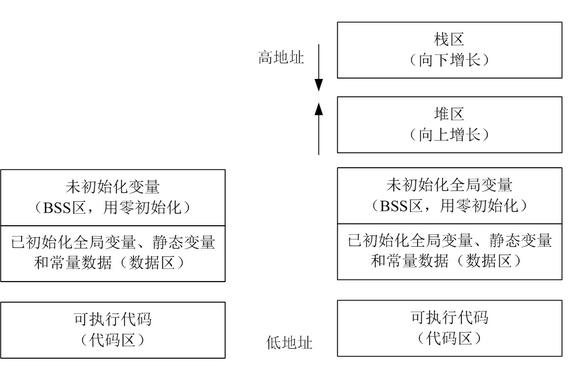
\includegraphics[width=0.6\linewidth]{app-in-disk-in-ram} %\pause
    \end{figure}
\end{frame}
%----------------------------------------------------------------------------------------

\begin{frame}
    \frametitle{OS实验内容}
    \framesubtitle{lab1: hello-world OS  软件}
    
    %    \begin{itemize}
    %        \item 直接与硬件交互的系统程序的编译运行
    %        \item 输出字符的方法
    %        \item 调试系统程序的方法
    %    \end{itemize}
    编译后的应用与运行时的应用
    \begin{figure}
        \centering
        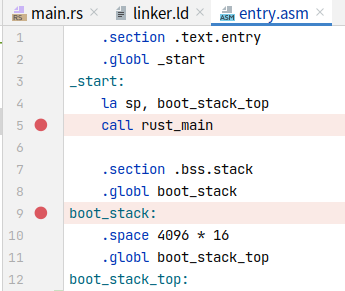
\includegraphics[width=0.45\linewidth]{entry-asm} %\pause
    \end{figure}
\end{frame}
%----------------------------------------------------------------------------------------

\begin{frame}
    \frametitle{OS实验内容}
    \framesubtitle{lab1: hello-world OS  软件}
    
    %    \begin{itemize}
    %        \item 直接与硬件交互的系统程序的编译运行
    %        \item 输出字符的方法
    %        \item 调试系统程序的方法
    %    \end{itemize}
    编译后的应用与运行时的应用
    \begin{figure}
        \centering
        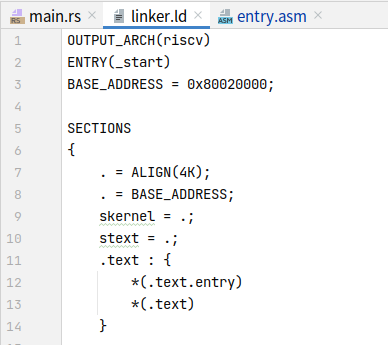
\includegraphics[width=0.45\linewidth]{linker-ld} %\pause
    \end{figure}
\end{frame}
%----------------------------------------------------------------------------------------

\begin{frame}
    \frametitle{OS实验内容}
    \framesubtitle{lab1: hello-world OS  软件}
    
    %    \begin{itemize}
    %        \item 直接与硬件交互的系统程序的编译运行
    %        \item 输出字符的方法
    %        \item 调试系统程序的方法
    %    \end{itemize}
    编译后的应用与运行时的应用
    \begin{figure}
        \centering
        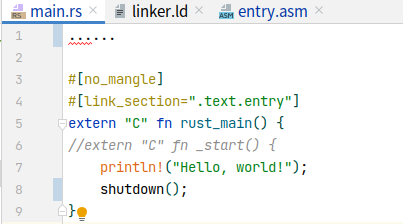
\includegraphics[width=0.6\linewidth]{main-rs} %\pause
    \end{figure}
\end{frame}

%----------------------------------------------------------------------------------------

\begin{frame}
    \frametitle{OS实验内容}
    \framesubtitle{lab1: hello-world OS  软件}
    
    %    \begin{itemize}
    %        \item 直接与硬件交互的系统程序的编译运行
    %        \item 输出字符的方法
    %        \item 调试系统程序的方法
    %    \end{itemize}
   % 编译后的应用与运行时的应用
    \begin{figure}
        \centering
        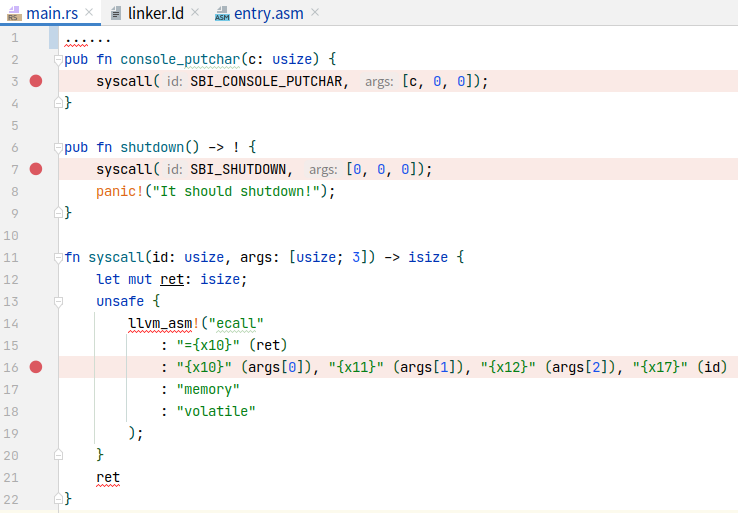
\includegraphics[width=0.65\linewidth]{sbicall} %\pause
    \end{figure}
\end{frame}

%----------------------------------------------------------------------------------------

\begin{frame}
    \frametitle{OS实验内容}
    \framesubtitle{lab1: hello-world OS  软件}
    问题
        \begin{itemize}
            \item 这个hello-world的执行环境包含啥?
            \item 在这个例子中操作系统是啥?
            \item 这个软件与我们通常的app相比,有哪些相同与不同的地方?
        \end{itemize}
     

\end{frame}
%----------------------------------------------------------------------------------------
\end{document}
